\documentclass[aps,prd,twocolumn,showpacs,superscriptaddress,groupedaddress,nofootinbib]{revtex4}  % for review and submission
\usepackage{graphicx}  % needed for figures
\usepackage{dcolumn}   % needed for some tables
\usepackage{bm}        % for math
\usepackage{amsmath,amssymb}   % for math
\usepackage{aas_macros}
\usepackage{multirow}
\usepackage{color}
\usepackage{verbatim}
\usepackage{times}
%what I add
\usepackage{tabu}
\usepackage{hyperref}
\usepackage{url}
\usepackage{microtype}
\usepackage[capitalise]{cleveref}
\usepackage[all]{hypcap}
\usepackage[toc,page]{appendix}
%
\newcommand{\mr}{\mathrm}
% avoids incorrect hyphenation, added Nov/08 by SSR
\hyphenation{ALPGEN}
\hyphenation{EVTGEN}
\hyphenation{PYTHIA}
\newcommand{\yr}{\ensuremath{\,{\rm yr}}}
\newcommand{\cm}{\ensuremath{\,{\rm cm}}}
\newcommand{\m}{\ensuremath{\,{\rm m}}}
\newcommand{\km}{\ensuremath{\,{\rm km}}}
\newcommand{\pc}{\ensuremath{\,{\rm pc}}}
\newcommand{\Mpc}{\ensuremath{\,{\rm Mpc}}}
\newcommand{\K}{\ensuremath{\, {\rm K}}}
\newcommand{\mK}{\ensuremath{\, {\rm mK}}}
\newcommand{\psr}{\ensuremath{\,{\rm sr}^{-1}}}
\newcommand{\Hz}{\ensuremath{\, {\rm Hz}}}
\newcommand{\kHz}{\ensuremath{\, {\rm kHz}}}
\newcommand{\MHz}{\ensuremath{\, {\rm MHz}}}
\newcommand{\erg}{\ensuremath{\,{\rm erg}}}
\newcommand{\eV}{\ensuremath{\,{\rm eV}}}
\newcommand{\keV}{\ensuremath{\,{\rm keV}}}
\newcommand{\Jy}{\ensuremath{\,{\rm Jy}}}
\newcommand{\Msun}{\ensuremath{{M_\sun}}}
\newcommand{\Lsun}{\ensuremath{{L_\sun}}}
\newcommand{\Zsun}{\ensuremath{{Z_\sun}}}
\newcommand{\tsec}{\ensuremath{{\rm s}}}
\newcommand{\nur}{\ensuremath{{\nu_R}}}
\newcommand{\nul}{\ensuremath{{\nu_L}}}
\newcommand{\los}{l.o.s.}
\newcommand{\tcb}{\textcolor{blue}}

\begin{document}
% The following information is for internal review, please remove them for submission
\widetext
% the following line is for submission, including submission to the arXiv!!
%\hspace{5.2in} \mbox{Fermilab-Pub-04/xxx-E}

\title{Cross Correlating 21 cm Intensity Mapping fields with Kinematic Sunyaev-Zel'dovich Effect: Probing Missing Baryons at $z\sim1-2$}
%\title{Cross Correlating Tidal Reconstructed 21 cm Signal with Kinematic Sunyaev-Zel'dovich Effect: A New Probe for Missing Baryons at $z\sim1-2$}
\input content/author.tex
\begin{abstract}
    The prominent defficiency of baryon contents in observations for $z\lesssim 2$ 
    and its close correlation with baryon distributions, galaxy feedbacks and 
    intergalactic medium conditions stand in the way of understanding structure 
    evolution. 
%To step aside from strong emission of galaxies and resolve 
 To study the distribution of diffusive 'missing baryons', 
a large scale oriented probe, 
the kinematic Sunyaev-Zel'dovich (kSZ) effect 
on cosmic microwave background, was proposed.
However, its faintness and lack of redshift require another 
signal to cross correlate with it. 
Previous proposals either require large sky galaxy spectroscopic surveys, 
or existing photemetric surveys combined with full ACTPol/CMB-S4 data to 
obtain persuasive results,
which is hard to achieve in next five years. 
In this paper, a new possibility of cross correlating 
    kSZ with HI density from 21cm Intensity Mapping surveys is discussed. 
    The high effeciency and low facility requirements of the surveys  
make it possible for several ongoing experiments, eg. CHIME, to achieve large sky coverage 
    and consistently measure $z\lesssim2$ sky in next few years. 
Assuming realistic facility conditions and noise scales, 
we find that after retrieving noise smeared 
    information on large scales with tidal coupling between scales, 
    a minimum of $~15$ S/N for both redshift 1 and 2 could be reached with CHIME + Planck. 
The fast construction of interferometers with longer baselines, eg. HIRAX, 
  may foster the S/N to reach $~50$ for redshift 2 with noise level of Planck.
\end{abstract}
\pacs{}
\maketitle

\section{Introduction}
For $z\lesssim 2$, large fractions of predicted baryon contents are missing in observations.  
The majority of them are believed to reside in warm-hot intergalactic mediums (WHIM) with typical temperature of $10^5$ K to $10^7$ K \cite{Pen1999,Soltan06}. 
High temperature and low density in the medium, 
as well as uncertainties in ionization states and metalicities, 
make it difficult to derive information from metal absroption lines. 
It is expected urgently for probes that not only trace the majority of the baryons, but also can be interpreted model-independently.

Among proposed probes, the kinematic Sunyaev-Zel'dovich (kSZ) effect \cite{Sunyaev72,Sunyaev80,Vishniac87} is a promising one.  
kSZ effect results from Compton scattering of cosmic microwave background (CMB) off free electrons. 
The radial velocity of electrons will give photon a Doppler shift 
and hence leads to a 
secondary anisotropy in CMB temperature.
%The kSZ signal could satisfy all three conditions listed before. 
%Consider kSZ as tracer has lots of advantages for this problem. 
It is an ideal probe to tackle the problem: 
First, it contributes from all the free electrons, indicating the distribution of $90\%$ of the baryons in ionized states,   
leaving alone only less than $10\%$ of baryons that 
reside in stars, remnants, atomic and molecular gases \cite{Fukugita04}. 
%
Second, the signal is mainly influenced by electron density and radial velocity, 
regardless the temperature, pressure and metalicity,  
so no extra assumptions are needed to estimate baryon abundance.  
%
Third, the peculiar velocity is dominantly related to large scale structures, 
therefore the signal is less biased towards local mass contraction, 
and more indicative about diffusive distributions.  

Attractive as it is, two drawbacks largely reduce the feasibility of harnessing kSZ signal.  
First, the signal is weak 
and hence suffers seriously from contaminations 
from primary CMB, facility noises, 
thermal SZ effect, CMB lensing, etc.  
Second, it is an integrated effect along line of sight, therefore, kSZ itself does not contain redshift information.

A straight-forward mitigation of the disadvantages is to cross correlate 
kSZ signal with another tracer, which has both large scale structure and redshift information. 
Previous work has proposed optical spectroscopic survey as an ideal tool \cite{Hand12,Shao11,Li14}. 
%However, lack of spectral lines in redshift $1.4-2.5$, and low survey speed has limited the application.  
However, first, it lacks detectable spectral lines in redshift $1.4-2.5$, 
therefore unable to consistently measure full $z<2$ sky. 
Moreover, kSZ signal is more prominent in higher redshift, 
while it is extremely inefficient for spectroscopic surveys to cover 
large sky area for $z>1$. 
Therefore this method is of no immediate access. 
%
Methods with lower facility requirements, such as 
cross correlating photo-z galaxies with kSZ \cite{Hill16,Ferraro16}, 
depends on models of velocity fields, 
and demands next generation CMB facilities to achieve 
convincing S/N.
%Optical spectroscopic surveys have been proposed as an ideal candidate. 
%Opitical spectroscopic surveys are one popular candidate. 
%However, they are not accessible on redshift $1.4-2.5$ 
%when all the lines are shifted away. 
%To consistently measure the sky from $z=0$ to $z=2$, we consider harness the H~I $21$ cm  line in radio band, which can also provide accurate redshift information.
%Rather than distinguishing individual galaxies, 
%we discuss the possibility of using integrated signals of each pixel 
%(intensity mapping) 

In this paper, a new possibility of cross correlating HI density field from 21 cm intensity mapping to kSZ signal is discussed. 
HI 21 cm spectra have accurate redshift information, 
and are fully accessible for $z\lesssim2$.  
%which enables us to reconstruct velocity field and 
%get better correlation with kSZ powerspectra. 
Intensity mapping survey, 
rather than distinguishing individual galaxies, 
integrates all weak signals in a pixel,  
which enables it to reach high S/N and scan large sky area 
in much shorter time. 
In the following few years, there will be several experiments 
producing data of large sky area for redshift $\lesssim2.5$ 
%CHIME \cite{2014SPIE.9145E..22B}, Tianlai \cite{2015ApJ...798...40X}, 
%HIRAX \cite{HIRAX} etc.
\cite{2014SPIE.9145E..22B, 2015ApJ...798...40X, HIRAX}.
%HIRAX \cite{HIRAX} etc.

However, as feasibility is usually traded from data quality, 
there are three main challenges for the upcoming H~I surveys  
in terms of cross correlation with kSZ. 
First, the integration of different signals will cause complicated foregrounds, 
which would smear the large scale structure in radial direction\cite{DiMatteo04,Masui13}. 
Second, the angular resolution is also supressed by the integration, 
droping information of small scale structure in transverse plane. 
Third, till now, the proposed experiments all work on interferometers, 
which drain the largest scale structure on transverse plane  
due to the finite length of the shortest baseline. 

%Since the kSZ signal is proposional to the convolution of density field and velocity field in Fourier space, 
On the other hand, the most prominate kSZ signals that could be distinguished from noises  
%is mainly from largest structure in radial direction 
are mainly from $k_z\lesssim0.1 h/Mpc$ in radial direction 
with $l < 100$ and $l \sim 1000-2000$. 
These modes are partly damaged in intensity mapping due to the three challenges. 
In this paper, we evaluate the 
influence of the incompelete modes
and partially recover the smeared large scale structures 
from their tidal influence on small scales\cite{2012:pen,2015:zhu}. 
Final correlation is presented against different conditions.

The paper is organized as follows: 
In section II, we demonstrate given a density field, how to correlate it with kSZ signal in a holographic way similar to \cite{Shao11}. 
In section III, the weights of different Fourier modes on generating kSZ signals 
are discussed and used to evaluate existing modes in 21cm intensity mappings. 
%then estimate which modes dominates the produced signal. 
In section IV, the method of 3D tidal reconstruction is introduced. 
Results of the reconstruction and cross correlation are presented in section V. 
And S/N is estimated via statistical error in section VI.
Finally we conclude at section VII.


Notes: 
Throughout the paper, We use the $z=1,2$ output of six $N$-body simulations from the
$\mr{CUBEP}^3\mr{M}$ code \cite{2013:code}, each evolving $1024^3$ particles in a $(1.2\mr{Gpc}/h)^3$ box. 
Simulation parameters are as follows: Hubble parameter $h=0.678$, baryon
density $\Omega_{b}=0.049$, dark matter density $\Omega_{c}=0.259$,
amplitude of primordial curvature power spectrum $A_s=2.139\times10^{-9}$ at 
$k_0=0.05\;\mr{Mpc}^{-1}$ and scalar spectral index $n_s=0.968$.


%=============================================
\section{Algorithm: kSZ Cross Correlation}
In this section, we present a holographic method 
to cross correlate kSZ with a density field, 
following \cite{Shao11}. 

\label{sec:kszRecon}
The CMB temperature fluctuations caused by kSZ effect is:
\begin{eqnarray}
\label{eq:ksz}
\Theta_{kSZ}(\hat n)\equiv\frac{\Delta T_{kSZ}}{T_{\mr{CMB}}}
=-\frac{1}{c}\int d\eta  g(\eta)  \bm{p}_\parallel\ ,
\end{eqnarray}
where $\eta(z)$ is the comoving distance at redshift z, $g(\eta)=e^{-\tau} d\tau/d\eta$ is the visibility function, $\tau$ is the optical depth to Thomson scattering, $\bm{p}_\parallel=(1+\delta)\bm{v}_\parallel$, with $\delta$ the electron overdensity, $\parallel$ indicates direction parallel to line of sight. 
We assume that $g(\eta)$ doesn't change significally in one redshift bin, 
and integrate $\bm{p}_\parallel$ along radial axis to get $\hat \Theta_{kSZ}$

Due to the cancellation of positive and negative velocity, direct cross correlation between kSZ signals and density contrast will vanish.
However, taking advantage of the known redshift, 
we could at most maintain the one to one multiplication between velocity field and density contrast   
by linearly calculating the peculiar velocity 
and generating a mock kSZ signal. 
%\cite{Shao11}.
%In this way, we can at most maximize the correlation.
The basic procedure is as follows:

Assume we have a density contrast field $\delta=(\rho-\bar{\rho})/\bar{\rho}$, where $\bar\rho$ is the average density of a certain redshift slice. 
%Detailed steps are as follows.

(1) Estimate the velocity field:

In linear region, the continuity equation goes like:
$\dot \delta+\nabla \cdot \bm{v}=0$, 
where $\bm{v}$ is the peculiar velocity and $\delta$ is the matter overdensity. 
%Therefore, we obtain an estimator of velocity distribution from the density contract $\delta$:
Therefore, linear velocity is estimated as: 
\begin{eqnarray}
	\label{eq:v}
\hat v_z(\bm{k})=i a H f\delta(\bm{k})\frac{k_z}{k^2}\,
\end{eqnarray}
where $f=d\mathrm{ln}D/d\mathrm{ln}a$, $D(a)$ is the linear growth function, 
$a$ is the scale factor, $H$ is the Hubble parameter.

$v_z \propto k_z/k^2$, indicating the most prominent signal comes from small k mode, which corresponds to large scale structure. 

(2) Filter the noise: 
The term $k_z/k^2$ in Eq.(\ref{eq:v}) will amplify noises in small k, 
which should be suppressed. 
\begin{eqnarray}
	\label{eq:wienerv}
\hat v_z^c(\bm{k})=\frac{\hat v_z(\bm{k})}{b(k_\perp,k_\parallel)}W(k_\perp,k_\parallel)\ ,
\end{eqnarray}
Bias $b=P_{\hat v_z,v_z}/P_{v_z}$, Wiener filter $W=P_{v_z}/(P_{\hat v_z}/b^2)$.

(3) Calculate 2D kSZ map following Eq.(\ref{eq:ksz}).

(4) Calculate correlation coefficients:

Quantify tightness of correlation with: 
\begin{eqnarray}
	r\equiv \frac{P_{recon,real}}{\sqrt{P_{recon}P_{real}}}\,
\end{eqnarray}
Where $\hat \Theta_{kSZ}$ is reconstructed signal 
and $\Theta_{kSZ}$ is original signal directly from simulations.


\section{Condition: kSZ + 21cm intensity Mapping}
In this section, we discuss the origin of kSZ signal 
on different structure scales, 
compare it with scales resolvable in 
ongoing 21cm Intensity Mapping experiments, 
and give an intuitive picture of the possibility and
 difficulty of the cross correlation.
 %==================================
\subsection{kSZ properties}
\begin{figure}[tbp]
\begin{center}
\includegraphics[width=0.48\textwidth]{figure/k3pd_k3pv_z1.eps}
\end{center}
\vspace{-0.7cm}
\caption{
    Illustrating weights of different scales after integration. 
    Demonstrated with data of redshift 1.
    (Top) The density variance $2\pi^2\Delta_\delta^2\equiv k^3P_\delta$. 
    (Bottom) The velocity variance $2\pi^2\Delta_{v_z}^2\equiv k^3P_{v_z}$. 
    (Red lines): Indicate most essential modes for generating kSZ signal in 
    $\ell\sim 500-3000$.
}
\label{fig:k3v}
\end{figure}

\begin{figure}[tbp]
\begin{center}
\includegraphics[width=0.48\textwidth]{figure/cmb_21cm.eps}
\end{center}
\vspace{-0.7cm}
\caption{
    (Top) Relative strength of angular powerspectrum between primary CMB, Planck noise in 217 GHz band, and kSZ effect in redshift 1 and 2.
    (Bottom) Available modes of density contrasts obtained 
    in realistic 21cm Intensity Mapping experiments, 
    with resolution of CHIME and high foregrounds ($R_\parallel=15$ h/Mpc) 
    in redshift 1. 
    $P_{21cm}$ is the remaining density powerspectrum after noise substraction; 
    $P_\delta$ indicates the powerspectrum of a intact density field.
}
\label{fig:cmb_21cm}
\end{figure}

%Since actual sky surveys can only resolve structures of certain scales, 
%it is essential to understand which scales contribute most to the kSZ signals. 
To understand what role each scale plays in generating kSZ signal, we write Eq.(\ref{eq:ksz}) in Fourier space. 

The finite box size of $1200$ Mpc only has notable influence on modes with $k\lesssim0.005$. 
It is safe to assume 
minus infinity to plus infinity 
integration on $z$ direction for small scale modes. 

Moreover, the term $a(z)H(z)f(z)$ in Eq.(\ref{eq:v}) does not vary much in one box, we assume it to be a constant for simplicity. 
Then the Fourier transformation is just the $k_z=0$ mode of the momentum 
$p_\parallel(\bm{k})$ in Fourier space. 
\begin{eqnarray}
    \label{eq:thetak}
    \Theta(\bm{\ell})&\equiv&\Theta({k}_x\chi,{k}_y\chi,0)\\
    &\propto&\int 
    d^3k^\prime\delta(\bm{\ell}/\chi-\bm{k}_\perp^\prime,k_\parallel^\prime) v_z(\bm{k^\prime})\nonumber
\subsection{21 cm Intensity Mapping Properties} 
\input content/noiseSubstraction.tex
\section{Algorithm: Cosmic Tidal Reconstruction}
\input content/tide.tex
\section{Results}
\input content/tideResult.tex
\section{Statistical error and s/n}
\input content/error.tex
\section{Conclusion}
\input content/conclusion.tex
\section{Acknowledge}
\input content/acknowledge.tex
\bibliographystyle{apsrev}
\bibliography{ksz}
\end{document}
